\documentclass{article}
\usepackage[utf8]{inputenc}
\usepackage{enumerate}
\usepackage{graphicx}
\usepackage{float}

\title{COL333: Assignment 3}
\author{Sachin 2019CS10722\\ Saurabh Verma 2019CS50129 }
\date{November 2021}

\begin{document}

\maketitle


Before implementing any AI learning we created a class called Map, that stores the map and checks for walls between two cells. We also created a class called State that stores the state parameters and has some useful functions required by different components of assignment.
Map class stores the map in the form of dictionary d (having walls) and 2 variables height and width. More of them will be explained inside the questions.
\section{Part A: Computing Policies}


\subsection{Formulation of the Taxi Domain as an MDP:}

We have created an MDP for the Taxi Domain formulation as described in the problem statement. We take the wall locations, position of depots, and width and height of the grid as input. Then we create an instance of the map class with these values and use in the MDP.
\begin{enumerate}[a)]
    \item
\textbf{State Space:\\}
We have created a class for the state. Each state in Taxi Driver MDP has four identifying features: the position of the taxi, position of the passenger,a boolean variable picked denoting whether passenger is picked by the taxi, and the destination. These are the variable describing the state.\\
Now the x position can take discrete values up to the width, y position can take up to the height. So the total number of values position of passenger and position of taxi can take is height*width. But when the boolean value of picked is true then position of taxi and passenger is same. And destination variable takes values equal to the number of depots. \\

So that makes the total number of variables to be :- \\
$w*h*w*h*d+w*h*d$\\ where,\\
h = height of map\\
w = width of map\\
d = number of depots\\
So state is $((x_1,y_1),(x_2,y_2),p,d)$ where $(x_1,y_1) = (x_2,y_2)$ if p is True.

\pagebreak

\item
\textbf{Transition Model: \\}Now the action in our formulation are (N, S, E, W, PICK, DROP). So the transition model is as follows.
\begin{itemize}
    \item T(s, DROP, s')=1
    \item T(s, PICK, s')=1
    \item This same applies to all the other direction(the x and y values get modified accordingly)
    \begin{itemize}
        \item T($(t_1,p_1,p,d),N,(t_2,p_2,p,d)$) = 0\\
        (Given that there exists a wall between two $t_1$ and $t_2$ otherwise:-)  
        \item T($((x,y),p_1,p,d),N,((x,y+1),p_2,p,d)$) = 0.85
        \item T($((x,y),p_1,p,d),N,((x,y-1),p_2,p,d)$) = 0.05
        \item T($((x,y),p_1,p,d),N,((x-1,y),p_2,p,d)$) = 0.05
        \item T($((x,y),p_1,p,d),N,((x+1,y),p_2,p,d)$) = 0.05
    \end{itemize}

    if p is True then $p_2$ = $t_2$ (taxi position in new state) else $p_2$ = $p_1$  in all above transitions.

\end{itemize}


\item \textbf{Reward Model:\\}The reward structure is as follows:
\begin{itemize}
    \item R($(d.pos,d.pos,True,d),DROP,(d.pos,d.pos,False,d)$) = 20
    \item R($s,DROP,(t_2,p_2,p,d)$) = -10\\
        (Given that $t_2 != p_2$)
    \item R($s,PICK,(t_2,p_2,p,d)$) = -10\\
        (Given that $t_2 != p_2$)
    \item All other transitions have a reward of -1
\end{itemize}
\end{enumerate}


\subsection{Implementing Value Iteration for the Taxi Domain:}
\begin{enumerate}[a)]
    \item We implemented the value iteration using max-norm distance in our code inside valueIteration() function in the MDP class. The value iteration took $\epsilon$ as the input. Also, the default value of $\gamma$ is set to be 0.9 but can be changed as specified.\\
    Answer to question asked in assignment:- 
    \begin{itemize}
        \item $\epsilon = $ 0.1 
        \item Number of iterations = 20
    \end{itemize}
    
    For the $\epsilon$ value of 0.1, the number of iteration the code took to converge is 20. We first tested our code different values of $\epsilon$ and following are the results of it:- 
    \begin{center}
        \begin{figure}[H]
        \hfill\includegraphics[width=9cm]{QA2a.png}\hspace*{\fill}
        \caption{Epsilon vs iteration Index}
        \label{fig:Epsilon vs iteration Index}
    \end{figure}
    \end{center}
    
    
    \item The plot of Max-norm distance vs Iteration index is given as follow: (The discount factors are given in the range [0.01,0.1,0.5,0.8,0.99] in that order)
    \begin{center}
        \begin{figure}[H]
        \hfill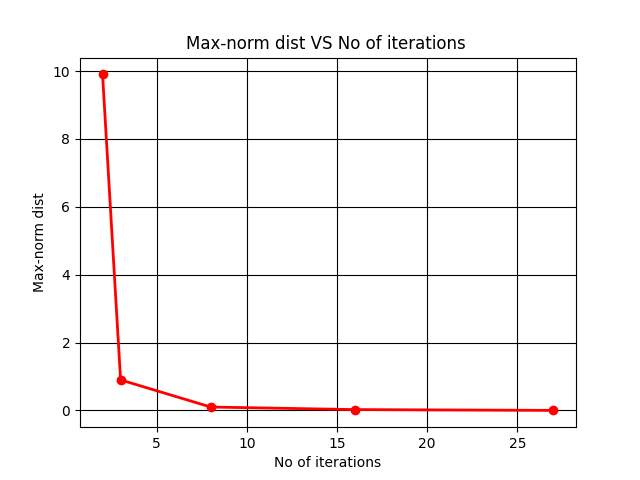
\includegraphics[width=9cm]{QA2b.png}\hspace*{\fill}
        \caption{Max Norm distance vs iteration Index}
        \label{fig:Max Norm distance vs iteration Index}
    \end{figure}
    \end{center}
    We used $\epsilon$ to be 0.1 in this part also.


    The max-norm distance is the amount of error we can incoperated in the values, that in a sense signifies the maximum difference from the optimal value. So as the number of iteration of convergence is increasing we are coming more and more close to the optimal value. Our estimates are improving further and further as we increase the number of iterations, hence the max-norm distance decreases. \\
    
    One another way to look at it is that as the max-norm distance decreases, the estimate value must be close to the optimal value itself, hence the number of iteration of convergence is more. 
    \item In this part we were asked to simulate the policy obtained using the value iteration once with $\gamma$ 0.1 and then with 0.99 with bound of 20 steps. Following are the results:- 
    
    \begin{itemize}
        \item \textbf{$\gamma$ = 0.1: } In this case the policy obtained are not optimal and taxi performs very poorely, very rarely it picks and drops the passenger in 20 states bound.
        \item \textbf{$\gamma$ = 0.99: } In this case policy obtained is optimal and taxi successfully picks and drops the passenger in required destination within 20 states.
    \end{itemize}

    This is because $\gamma$ denotes the discount factor of algorithm, that is quantifier of importance given to Values of states that are visited later (far off states) so if $\gamma$ is kept low, then there is less transfer of imformation from one state to another (because there is more attenuation) and hence poor learning.

\end{enumerate}
\subsection{Implementing Policy Iteration for the Taxi Domain:}
\begin{enumerate}[a)]
    \item To implement the policy evaluation step, we have two options; one is the exact method in which we create linear equations in variables equal to the number of the total state and get the exact utility value of the various states. The other is the approximate method which runs an update on the states until the value converges.
The first method mentioned is called Linear Algebra Method, the second one is the Iterative method. We have implemented them both. \\

The linear algebra method takes O($n^3$) time for policy evaluation, where n is the number of states. If the transition model given to us is sparse, meaning that each state transition leads to only a small number of states, then the Linear algebra method is preferred because then the solution is obtained faster. The linear Algebra method is preferred when our state space is small. For larger state space, O($n^3$) becomes too much overhead, so iterative method is preferred
    \pagebreak
\item The graph comes out as following for different values of the discount factor.
    \begin{center}
        \begin{figure}[h]
\hfill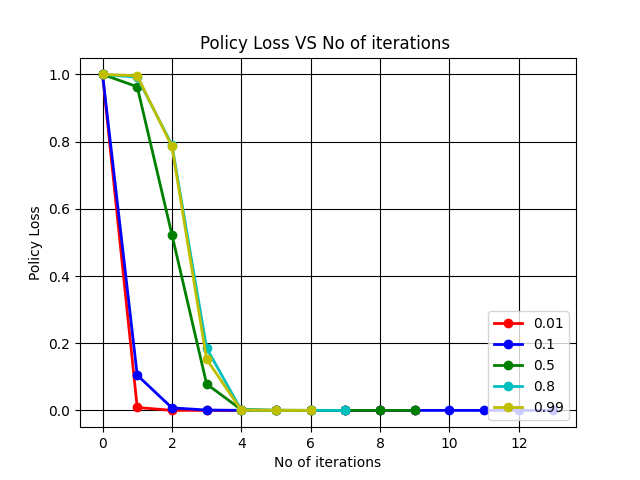
\includegraphics[height=6.5cm]{QA3b.png}\hspace*{\fill}
    \caption{Policy Loss}
    \label{fig:Policy Loss}
\end{figure}
\end{center}

\pagebreak

\section{Part B: Incorporating Learning}


\subsection{Implementing the approaches to learn the optimal policy:}
In this part we had to implement the Q learning and SARSA reinforcement learning techniques with different exploration methods.\\
For doing that we made a general function that on changing parameter becomes required algorithm. This function takes $\epsilon$ and $\alpha$ as
parameters and learns the optimal Q table. Initially we started with Q table with all values 0 and performed n number of iterations of episodes. In 
each episode, starting from a random state we keep on moving to next state by performing action depending upon exploration technique and updating Q value depending on
algorithm (Q learning or SARSA) by using the reward got upon performing that action untill we reached terminal state. \\

Learning techniques:- 
\begin{itemize}
    \item \textbf{Q learning: }  This is an off policy algorithm, where Q table is updated using the following formula:-\\ 
        $ Q(s,a) = (1-\alpha)Q(s,a) + \alpha(R(s,a,s') + \gamma max_{a'}Q(s',a'))$
    \item \textbf{SARSA: }  This is an on policy algorithm, where Q table is updated using the following formula:- \\
    $ Q(s,a) = (1-\alpha)Q(s,a) + \alpha(R(s,a,s') + \gamma Q(s',a'))$\\
    where $a'$ is some random action from $s'$\\
\end{itemize}

Exploration techniques:- 
\begin{itemize}
    \item \textbf{e-greedy: } Any random action with probability e otherwise best action according to Q table.
    \item \textbf{exploration decay: } Any random action with probability e/$\sqrt{i}$ (where i = iteration number) otherwise best action according to Q table.
\end{itemize}


\subsection{Number of iterations VS Discounted reward:}
In this part we needed to plot Number of iterations VS Max-norm dist graph for all the algo in part 1. For that we first find the Policy by varying number of iterations and then found 
sum of discounted rewards for 500 random states (for better results) and then average out the reward. And then plotted the graph between number of iteration and discounted reward sum. Same is repeated for all algorithms.\\
Following are the results:-


\begin{center}
    \begin{figure}[H]
    \hfill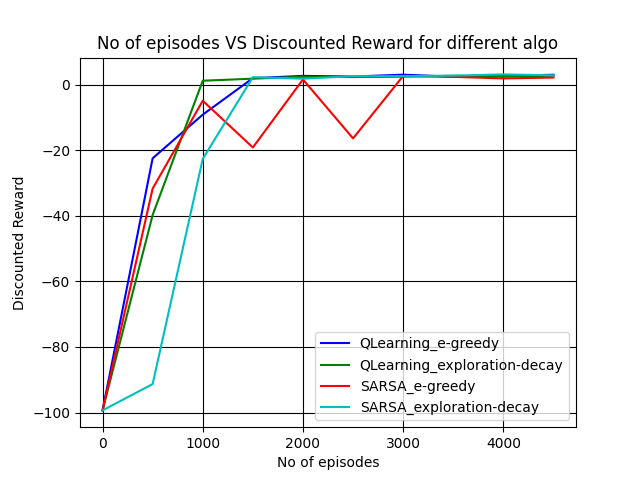
\includegraphics[width=9cm]{QB2.png}\hspace*{\fill}
    \caption{No of episodes VS Discounted Rewards for different Algo}
    \label{fig:No of episodes VS Discounted Rewards for different Algo}
\end{figure}
\end{center}

\textbf{Analysis:\\ }
Since Q learning is a off policy algorithm, it assumes that greedy policy is followed till now (but infact it is not), and takes the best action availabe, as best action is taken at each state while learning the number of negative rewards are less, whereas SARSA is an on 
policy, i.e. it takes some random action for updating its Q table. But by doing so in the learning process there are more negative rewards in it. So, initially when we let the agent train for less number of iterations we can see Q leaning approaching to more positive rewards faster than 
SARSA (both the approaches of exploration).\\

Now, coming to the choice of exploration technique, $\epsilon$ greedy simply takes random state with probability of $\epsilon$ at each point of the training, but ideally we should focus on exploitation of current policy once we have explored most of the states (i.e. in the later part of training), 
that is what is done in exploitation decay. In our implementation, exploration decays with the factor of $\sqrt{i}$ where i is number of states agent have been so far (repeated counting allowed). So, as evident from graph exploration decay version of both Q learning and SARSA converge to positive rewards faster than 
their $\epsilon-$greedy versions.\\

So combining both the effects Q learning with exploration decay is the best algorithm (same can be seen in graph, it converges fastest).  


\subsection{Execution using learned policy:}
In this we started from any random start state used the policy values learned using Q learning with exploration decay to perform action at any state. So basically 
we simulated the episode using learned actions. This is done on 5 random start states. Following are the results:-

\begin{itemize}
    \item The taxi is able to successfully pick the passenger and then drop it at the correct destination in less than the bound set(500) on steps.
    \item There are stochastic behaviour in next state. Sometimes when taxi takes action North, still it moves in direction other than North.
    \item But taxi is able to overcome that probabilistic behaviour and able to perform optimally from any given state.
\end{itemize}

\subsection{Analysing effect on policy by changing $\epsilon$ and $\alpha$:}
In this we needed to plot graph of part 3 by changing $\alpha$ and $\epsilon$ for Q learning with e-greedy. Following are the results:- 

\begin{enumerate}
    \item \textbf{$\alpha$ = 0.1 and varying $\epsilon$: }
    
    \begin{center}
        \begin{figure}[H]
        \hfill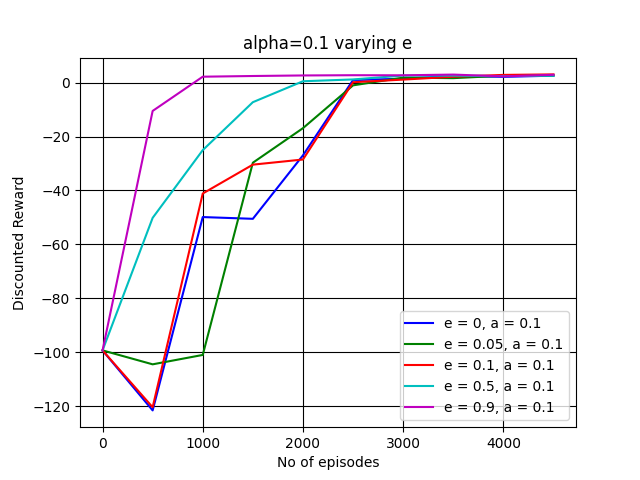
\includegraphics[width=9cm]{QB4_alpha=0.1.png}\hspace*{\fill}
        \caption{alpha = 0.1 and varying epsilon}
        \label{fig: alpha = 0.1 and varying epsilon}
    \end{figure}
    \end{center}

    It can be seen from the graph that as $\epsilon$ is increased, rewards converges in lesser number of iterations. This is quite imperative as 
    $\epsilon$ is the probability with which we are exploring states and as more and more states are observed, changes in Q values from far off state travels 
    faster. But there is a tradeoff in time taken per episode. Since we are giving more priority in exploring than exploiting current state, terminal state is 
    reached in larger time.

    \item \textbf{$\epsilon$ = 0.1 and varying $\alpha$: }
    
    \begin{center}
        \begin{figure}[H]
        \hfill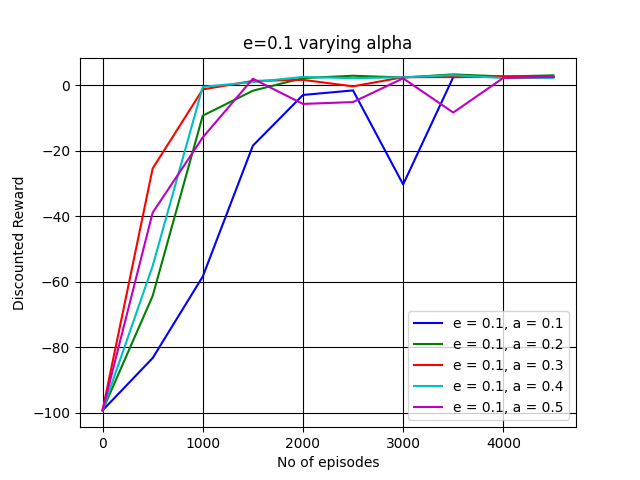
\includegraphics[width=9cm]{QB4_e=0.1.png}\hspace*{\fill}
        \caption{epsilon = 0.1 and varying alpha}
        \label{fig: epsilon = 0.1 and varying alpha}
    \end{figure}
    \end{center}

    It can be seen from the graph that from $\alpha$ = 0.1 to $\alpha$ = 0.4, convergence in reward is acheived in lesser number of iterations, also fluctuations in reward decreases  (graph moves towards increasing behaviour). But for 
    $\alpha$ = 0.5, again flutuations can be seen and number of iterations required for convergence increased again. This is because $\alpha$ is the learning factor that is the weight by which we are giving priority to last update compared to value 
    obtained so far. So initially when $\alpha$ is less, since we give lesser weight to values that we get, reward information is not correctly propagated. Whereas once we have reached the best $\alpha$ (that balances both last update and 
    previous value) and increase $\alpha$ further then it will also result in poor behaviour because higher $\alpha$ means we are just relying on last update, not on value got till now. So basically $\alpha$ is simply quantifier of value to noise ratio and should be adjusted accordingly.

    
\end{enumerate}


\subsection{Testing on larger grid:}
For this part we were required to test out best algorithm on 10*10 grid provided. For that we first created the grid using the method explained in first part, then we calculated the optimal Policies for all 8 destinations using all 4 algorithm(10,000 iterations) and stored them. Then we found discounted reward sum on 500 instances of problem and took average of that.
Here are the resuls of all the 4 policies:- 
\begin{itemize}
    \item \textbf{Q Learning with e-greedy: } -9.39
    \item \textbf{Q Learning with exploration decay: }  -8.32
    \item \textbf{SARSA with e-greedy: }  -18.70
    \item \textbf{SARSA with exploration decay: } -8.61
\end{itemize}

Hence best algorithm is Q Learning with exploration decay.\\

Please note that average reward is coming out to be negative even for the best policy, this is because our map is big and shortest path from taxi's initial position to passenger's source to passenger's destination can have
more than 20 grid cells, so there are some instances (one such instance is shown below) where even if we are lucky enough to get into to desired cell for every stochastic action then also we will get negative reward. Hence in average the net discounted reward sum is negative.
Also as we have averaged out the result on 500 random episodes, the result is reliable and evident of the policy itself.


\begin{center}
    \begin{figure}[H]
    \hfill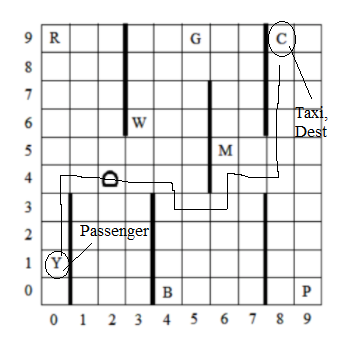
\includegraphics[width=7cm]{instance.png}\hspace*{\fill}
    \caption{Instance having shortest path length = 36 (best reward sum = -17.8)}
    \label{fig: Instance having shortest path length = 36 }
\end{figure}
\end{center}
\end{enumerate}
\end{document}
